\chapter{Motion planning}

\section{Existing local planner algorithms}
\label{chap:existing_local_planner_algorithms}
After building a map of the static and dynamic objects surrounding the vehicle, the next step is motion planning, which consists of two sub-tasks - global trajectory planning and local obstacle avoidance. As a result of global planning, a trajectory is created that - without taking the moving obstacles into consideration - leads the car to the target configuration, without making it collide with any static objects in the way. Local obstacle avoidance takes this trajectory as its input, and updates the car's actuators (acceleration and steering) to follow this trajectory, while also preventing collisions with dynamic objects.
As a part of my diploma project, I implemented the latter, a local obstacle avoidance algorithm, that relies on the previously created static and dynamic maps, and gets its input trajectory from a global planner node\footnote{Implementing a global motion planner was not part of my diploma project, but is considered a necessary condition for the local planner to work properly.}. According to \cite{DynamicMotionPlanningSurvey}, there exists a wide range of local planner algorithms, and they can easily be grouped by their complexity:

\begin{itemize}
  \item Velocity-based methods, most of the times combined with the dynamic window approach
  \item Predictive and probability-based methods
  \item Complex methods based on visual detection and AI
  \item Other methods
\end{itemize}

Out of these methods, velocity-based algorithms are by far the most popular, due to their being relatively easy to comprehend and implement and because of their low hardware requirements. As the mapping node and the local planner that I designed need to run on a processor with limited resources, I also chose a velocity-based obstacle avoidance method, using velocity obstacles, with dynamic windowing.

\section{Method}

The planner algorithm I implemented uses velocity obstacles to determine which configurations of the car are safe. Velocity obstacle methods (descibed in \cite{VelocityForbiddenMap} and in \citep{VelocityObstacles}) are based on the following statement: \textit{Assuming a given a given vehicle configuration (position, orientation, speed and wheel angle), the time until collision with a given static or dynamic object in the map can be calculated.} Therefore, velocity obstacle-based methods calculate this collision time for all surrounding objects and for all vehicle velocities. thus creating a velocity obstacle map, or forbidden velocity map (also referred to as dynamic velocity space in \cite{DynamicMotionPlanningSurvey}). Using the dynamic window approach is advised in this step,as it filters out non-reachable velocities before collision-time calculations, thus decreasing the execution time of the algorithm.
Given this velocity obstacle map, the algorithm has a basic knowledge of the reachable velocities and their level of safety. These safety levels provide a good starting point for further calculations, trajectory and collision estimations. My algorithm converts the forbidden velocity map's collision times to safety factors, but also takes the destination point's position and the target speed into consideration when selecting the next actuator outputs.
The next graph shows all the sub-tasks of the local trajectory planner algorithm.

\tikzset{
     base_node/.style = {rectangle, rounded corners, draw=black,
                         minimum width=4.5cm, minimum height=1cm,
                         text centered, font=\sffamily},
  inout_node/.style        = {base_node, fill=blue!30},
  update_node/.style   = {base_node, fill=orange!15},
  dynamic_node/.style  = {base_node, fill=red!30},
  static_node/.style   = {base_node, fill=yellow!30},
  velo_obs_node/.style = {base_node, fill=green!30},
  decoration={brace},
  tuborg/.style={decorate},
  tubnode_left/.style={midway, left=2pt},
  tubnode_right/.style={midway, right=2pt}
}

\begin{figure}[!ht]
    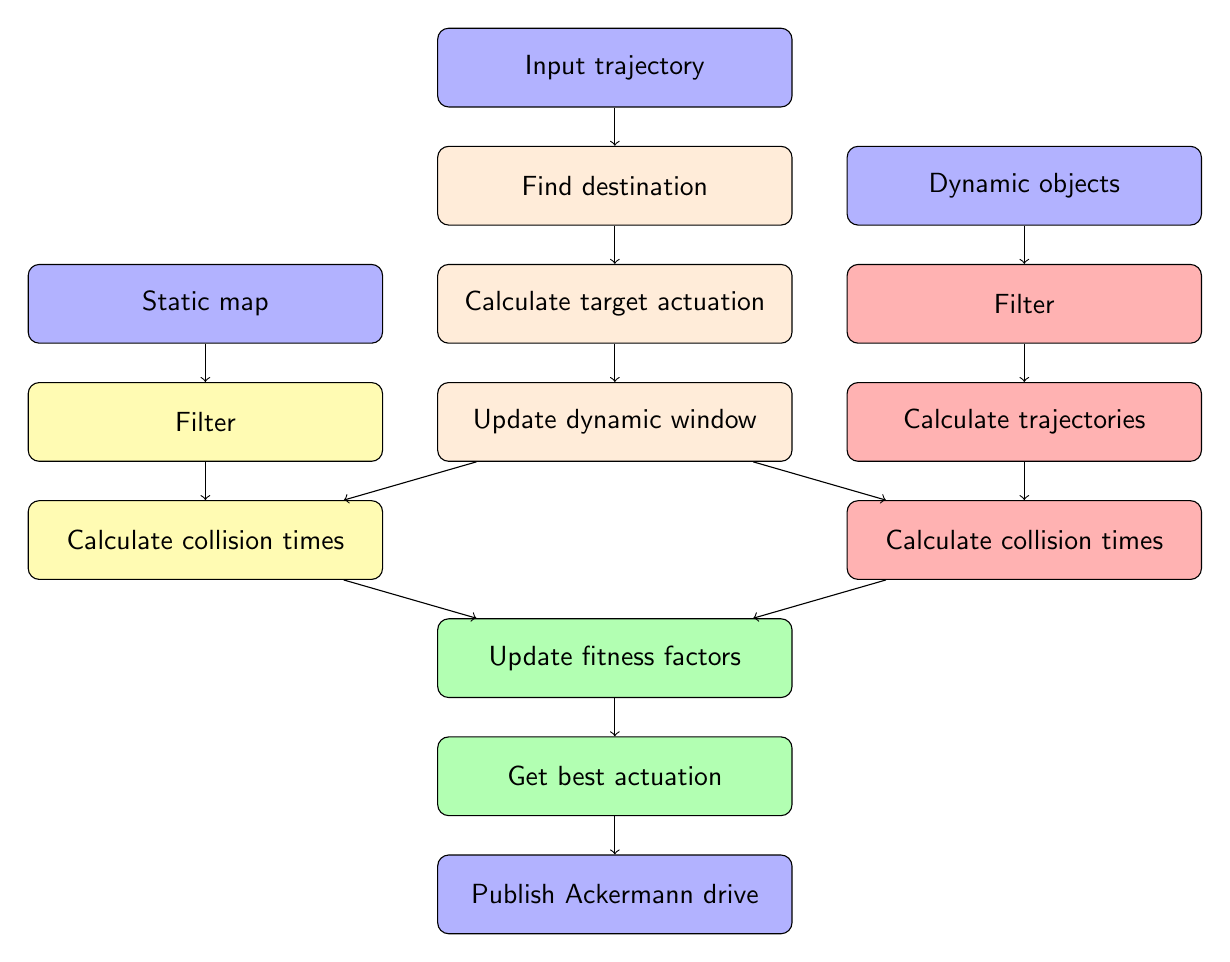
\begin{tikzpicture}[
            node distance=1.5cm,
            every node/.style={fill=white, font=\sffamily}, align=center]
        % Input nodes
        \node (static_map)      [inout_node, yshift=-3cm]                              {Static map};
        \node (trajectory)      [inout_node, xshift=5.2cm]                             {Input trajectory};
        \node (dynamic_objects) [inout_node, xshift=10.4cm, yshift=-1.5cm]             {Dynamic objects};
        % Update nodes
        \node (find_dest)       [update_node, below of=trajectory]                     {Find destination};
        \node (calc_target_act) [update_node, below of=find_dest]                      {Calculate target actuation};
        \node (update_window)   [update_node, below of=calc_target_act]                {Update dynamic window};
		% Static nodes
        \node (static_filter)   [static_node, below of=static_map]                     {Filter};
        \node (static_calc_col) [static_node, below of=static_filter]                  {Calculate collision times};
		% Dynamic nodes
        \node (dynamic_filter)  [dynamic_node, below of=dynamic_objects]               {Filter};
        \node (dynamic_traj)    [dynamic_node, below of=dynamic_filter]                {Calculate trajectories};
        \node (dyn_calc_col)    [dynamic_node, below of=dynamic_traj]                  {Calculate collision times};
        % Velocity obstacle nodes
        \node (fitness_factors) [velo_obs_node, below of=update_window, yshift=-1.5cm] {Update fitness factors};
        \node (get_best_act)    [velo_obs_node, below of=fitness_factors]              {Get best actuation};
        \node (acker_drive)     [inout_node, below of=get_best_act]                    {Publish Ackermann drive};
        % Static connections
        \draw[->]      (static_map) -- (static_filter);
        \draw[->]   (static_filter) -- (static_calc_col);
        % Update connections
        \draw[->]      (trajectory) -- (find_dest);
        \draw[->]       (find_dest) -- (calc_target_act);
        \draw[->] (calc_target_act) -- (update_window);
        \draw[->]   (update_window) -- (static_calc_col);
        \draw[->]   (update_window) -- (dyn_calc_col);
        % Dynamic connections
        \draw[->] (dynamic_objects) -- (dynamic_filter);
        \draw[->]  (dynamic_filter) -- (dynamic_traj);
        \draw[->]    (dynamic_traj) -- (dyn_calc_col);
        % Velocity obstacle connections
        \draw[->] (static_calc_col) -- (fitness_factors);
        \draw[->]    (dyn_calc_col) -- (fitness_factors);
        \draw[->] (fitness_factors) -- (get_best_act);
        \draw[->]    (get_best_act) -- (acker_drive);
    \end{tikzpicture}
    \caption{Motion planning method}
    \label{motion_planning_method}
\end{figure}

The diagram consists of 4 subgraphs - these are also marked on the diagram with different colors. The first (and shortest) one is about the method of reducing the size of the static map by filtering out those points that are not needed for the trajectory planning. The second one shows that for dynamic objects, trajectory calculation is also necessary besides filtering. The third describes the environment-independent sub-tasks of the algorithm - finding the next destination point, updating the target actuation and the dynamic window. And the last subgraph (populating the bottom area of the graph) contains the main planning logic. The next sections are going to explain these subgraphs in detail.

\section{Static velocity obstacle map}
\label{chap:static_velocity_obstacle_map}

\subsection{Filtering static points}

\subsection{Static collision times}

\section{Dynamic velocity obstacle map}
\label{chap:dynamic_velocity_obstacle_map}

\subsection{Filtering dynamic objects}

\subsection{Trajectory calculation}

\subsection{Dynamic collision times}

\section{Velocity obstacle map evaluation}
\label{chap:velocity_obstacle_map_evaluation}

\subsection{Fitness factors}

\subsection{Best actuation}

\subsection{Publishing Ackermann driving control}
